\chapter{Real Time Systems}

\newpage
\section{RTOS}
%- have image comparing normal and RTOS. 
%- when ever you have time you can have the standard linux kernal on top of the RTLinux and run it as a task.
A realtime OS needs to be \textit{Determinism}, we want the ability to control
the sequence of execution. \textit{Responsiveness}, i.e. there should be short
interrupt latency as well as fast context switching. It should also have a \textit{small
footprint}, i.e. use little storage. Some other requirements are \textit{Support for timely concurrent processing}, 
which allow real-time, multi-tasking, and synchronization. Also, \textit{User control over OS policies}, 
which allow CPU scheduling and memory management.

\begin{figure}[H]
\centering
\begin{subfigure}{.5\textwidth}
  \centering
  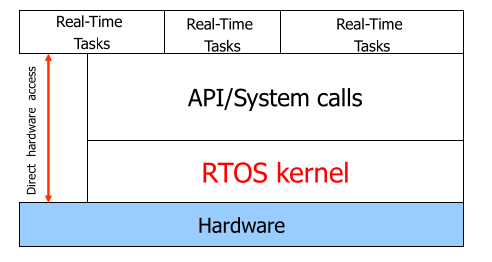
\includegraphics[width=\linewidth]{\imagesPath/rtos.png}
  \caption{RTOS}
  \label{fig:rtos}
\end{subfigure}%
\begin{subfigure}{.5\textwidth}
  \centering
  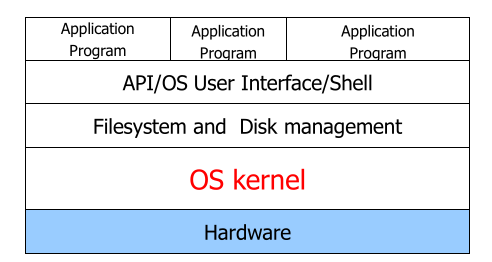
\includegraphics[width=\linewidth]{\imagesPath/other_os.png}
  \caption{Other OS}
  \label{fig:other_os}
\end{subfigure}
\caption{Realtime OS and other OS, \cite{RTOS, l2, p6}}
\label{fig:test}
\end{figure}

\subsection{Time management}
The hardware has a timer which interrupts the processor at a fixed rate (i.e. \textit{Time Interupt}). Each time interupt is called a system \textit{tick}.
For each time interrupt routine the cycclic task will starte again when a period has past.
%- time interrupt routine, for the cycle tasks it, the curnal has a time/timmer that then restart the task when a period has past.

\subsection{Task mangement}
Timming constrained, time-driven.

Periodic tasks described with 3 parameters (C,D,T) where
\begin{itemize}
\item C = resource budget
\item D = deadline
\item T = period (e.g. 20ms, or 50HZ)
\end{itemize}
Often D=T, but it can be D<T or D>T

\textit{Time-driven} means that the task is depending on time, e.g. periodic tasks. 
There is also \textit{Event-driven}, which are instead dependent on a interupt.
\begin{itemize}
\item C = resource budget
\item D = deadline
\item T$_{min}$ = minimum interarrival time
\end{itemize}

It is not the end of he world the the deadline is greater
then the period since it want relay effect the system in a negative way.
But it is easier to conceptualize and work with if the deadline is within the period.

\newpage
\begin{figure}[H]
    \centering
    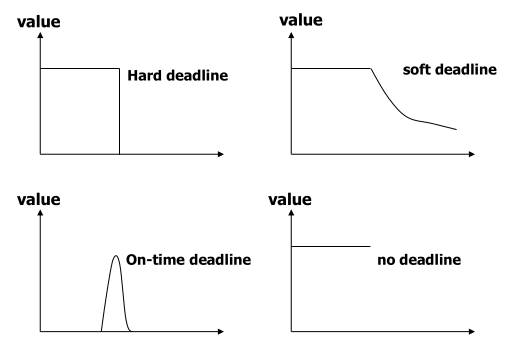
\includegraphics[width=10cm]{\imagesPath/timing_constraints.png}
    \caption{Timing Constraints, \cite{RTOS, p.21}}
\end{figure}


Task states
\begin{itemize}
\item Ready
\item Running
\item Waiting/blocked/suspended \ldots
\item Idling
\item Terminated
\end{itemize}

\textit{TCB} (Task Control Block) is the meta data of the task.


\subsection{Interrupt handling}
\begin{figure}[H]
    \centering
    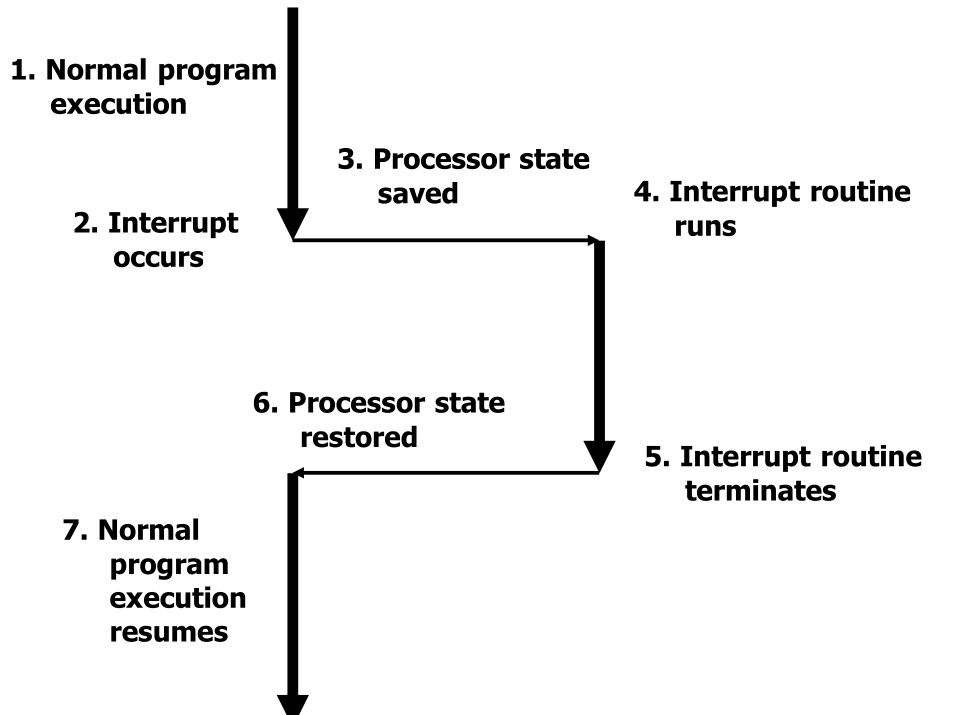
\includegraphics[width=10cm]{\imagesPath/handling_an_interrupt.png}
    \caption{Handling an Interrupt, \cite{RTOS, p.29}}
\end{figure}


\subsection{Memory management}
Memory is handled tru the standard method with Block-based, Paging, hardware mapping for protection.
For some cases there are no virtual memory, i.e. Lock all pages in main memory.
Several embedded RTS does not have memory protection since it is not neeeded for a correctly design system. 


\subsection{Exception handling}
\textit{Exceptions} e.g missing deadline, running out of memory, timeouts, deadlocks, divide by zero, etc.
Watch-dog we create a monitor that looks at some result that is a seperate tasks.

\subsection{Task scheduling}
Most importent.
Sort the READY queue acording to
\begin{itemize}
\item Priorities (HPF)
\item Execution times (SCF)
\item Deadlines (EDF)
\item Arrival times (FIFO)
\end{itemize}
Classes of scheduling algorithms
\begin{itemize}
\item Preemptive vs non preemptive
\item Off-line vs on-line
  \begin{itemize}
  \item Static vs dynamic: Static has less overhead than dynamic since a dynamic scheduling algorithm like EDF has to constantly check which deadline is the closes.
  However dynamic like EDF is the optimal scheduling algorithm for single core preemptive processor. 
  Static is less flexible as it can not change during runtime to better fit the task set.
  Dynamic doesn't need to save a static schedule or priority ordering of the task set, but static need until the hyper period.
  \end{itemize}
\end{itemize}

Interrupt it is a vector of bits so 8 bit has 8 interrupts
and the first has the highest priority and the last is the lowest.

\subsection{Task synchronization}
Synchronization primitives can be used such as \textit{spinlock} and \textit{semaphores}.

Potential synchronization issues that can occurs are \textit{deadlock}, \textit{livelock}, 
\textit{starvation}, which can be caused by critical sections. Also \textit{priority inversion} a higher-priority job can block a medium-priority job.


\subsection{Types of tasks}
\begin{itemize}
  \item Sporadic tasks: it reoccurs in random instances and has hard deadlines.% is a time-driven meaning that it has execution time $C_i$, deadline $D_i$, and minimum interarrival time $T_{minimum}$.
  \item Asynchronous periodic tasks: instead have $O_i$ aka offset/ the arrival time, $C_i$, $D_i$, $T_i$.
  \item synchronous periodic tasks: All tasks arrive at he same time.
\end{itemize}
SAS: the hardest sequence that is a set of sporadic tasks is synchronous and then release as early as possible.
Meaning that to analyze sporadic task we treat them as synchronous periodic tasks.


\section{ADA}
Standard for automotives \textbf{AUTOSAR}.


\begin{figure}[H]
    \centering
    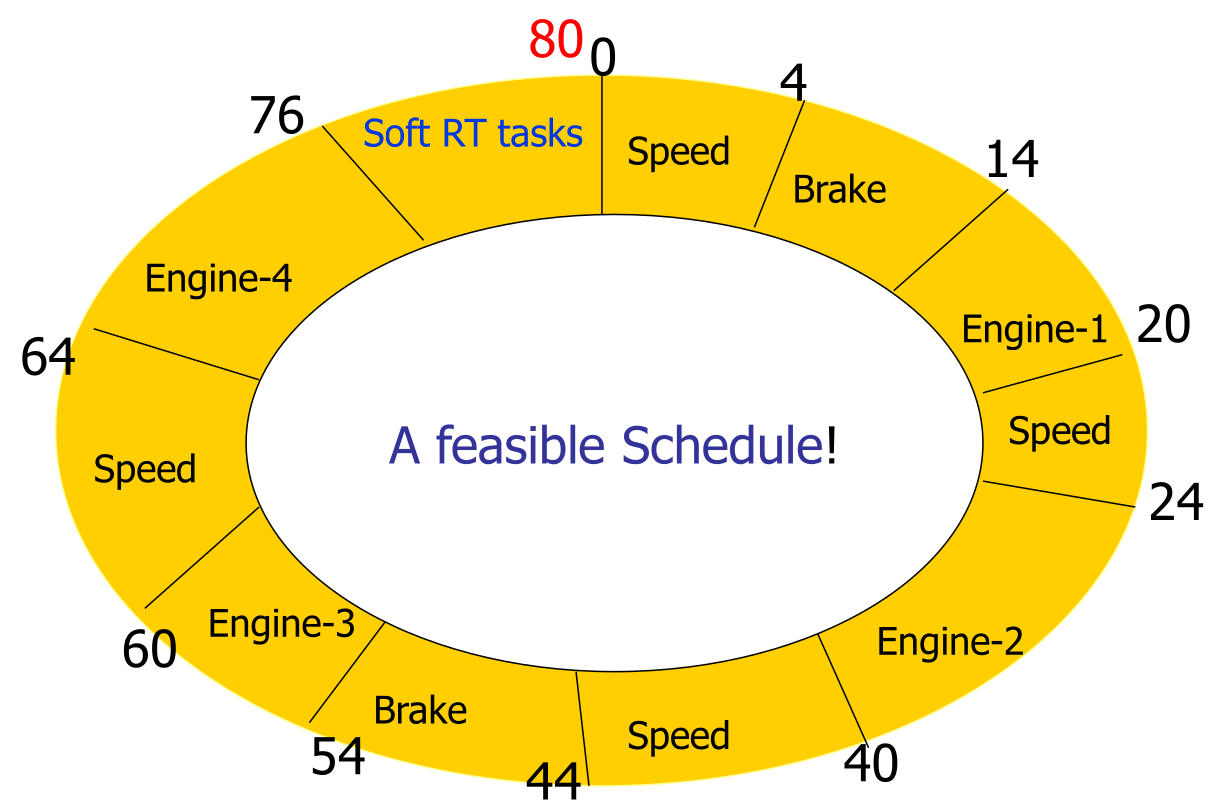
\includegraphics[width=10cm]{\imagesPath/feasible_schedule.png}
    \caption{Handling an Interrupt, \cite{RTOS, p.29}}
\end{figure}

%Clyclic execution vs multitasking. It is the worst case senario so that is why we can have it static.

\textit{Worst-Case Response Time} (WCRT). A task might not finish its execution due to \textit{prempty}, i.e. remove the task from exectuing and then let the another task get the computing resources. 
If we have a cold cash then it will take longer, and therefore need to be taken into consideration when calculating WCET.

A job is a execution of a task. A arraying time, C computing time, D deadline.

The delay will cause a delay for at least a specified time interval. The delay until causes a delay until an absolute wake-up time.

For tasks ADA let you specify entries which is defined in the a select statement.
It is often you have the select statements in a loop as it should be possible to call
a task entry multiple time. However, eventhough it is a loop it doesn't contently run over and over again.
It instead wait until someone calls the entry.


\section{Sheduling}
% Lecture 4?
\textbf{Classical scheduling theory} (e.g., in operations research)
generally deals with \textit{finite} processes (job-shop, flow-shop \&c.)
to \textit{optimize} some metric.

\textbf{Real-time scheduling theory}
generally deals with \textit{infinite} processes (control loops \&c.)
to \textit{guarantee} a safety specification.

\begin{itemize}
  \item Task models: Formalisms to specify workload and timing constraints.
  \item Scheduling algorithms: Run-time strategies for scheduling workload.
  \item Analysis: Offline methods for proving timing safety.
\end{itemize}

A job $j_i$ is geven by a triple $(A_i,C_i,D_i)\in\mathcal{N}^3$, where
\begin{itemize}
  \item $A_i$ is the arrival time (or release time),
  \item $C_i$ is the  worst-case execution time (WCET), and 
  \item $D_i$ is the deadline.
\end{itemize}


\begin{figure}[H]
    \centering
    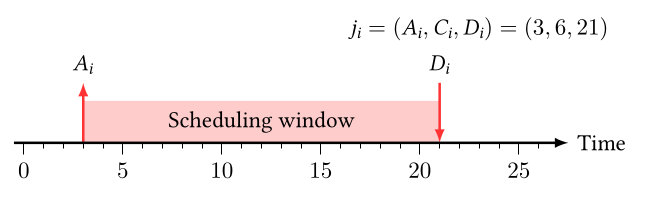
\includegraphics[width=10cm]{\imagesPath/scheduling_window.png}
    \caption{Scheduling window, \cite{05, p.7}}
\end{figure}

We are \textbf{assuming} 1. All jobs are independent, 2. A single processor, and 3. Fully preemptive or non-oreemptive scheduling.

Context switching
\begin{itemize}
  \item \textit{Preemptive}: allow jobs to be paused and resumed later.
  \item \textit{Non-preemptive}: dont allow context switching, the job who has cpu time will run until the end.
\end{itemize}

Important definitions
\begin{itemize}
  \item \textit{Schedualability}: iff the sheduling algorithm shedules the set of jobs without deadline misses.
  \item \textit{Feasibility}: iff there exists a sheduling algorithm that is schedulable.
  \item \textit{Optimality}: iff all sets of feasible shedules are also schedulable.
\end{itemize}


Test definitions:
\begin{itemize}
  \item \textit{Sufficient test}: iff by passing the test means that the system is schedulable.
  \item \textit{Necessary test}: iff by failing the test means that the system is unschedulable.
  \item \textit{Exact test}: iff sufficient and necessary.
\end{itemize}

Schedualability test we compute that the response time is within all deadlines, then it is schedulable.
EDF can be used to test since if it not feasible with EDF it is the jobs are not schedulable.
Preemptive EDF, the first argument is when the task arrives.

\begin{itemize}
  \item \textit{Implicit deadlines}: if $D_i = T_i$ for all $\tau\in\mathcal{J}$. Is when the deadline and period are the same.
  \item \textit{Constrained deadlines}: if $D_i \leq T_i$ for all $\tau\in\mathcal{J}$.
  \item \textit{Arbitrary deadlines}: if $D_i$ and $T_i$ are unrealated.
\end{itemize}
 
Other terminology:
\begin{itemize}
  \item \textit{Priority ordering}: tells us who has the highest priority.
  \item \textit{Critical instant schedule}: shows what task have the resorces, and it is used to determine if deadlines are meet.
  \item \textit{Utilization}: see equation. executing time / period $ (C_i / T_i)$.
  \item \textit{Higher periodicity}: hp\{$\mathcal{J}$\}.
\end{itemize}


\subsection{Scheduling algorithms}
A static schedule is a schedule for a hyper period which will then reapet over and over again. A static priority is a priority that want change.
\begin{itemize}
  \item Dynamic priotiry: the priority change during run time
  \begin{itemize}
     \item EDF: The task with the earliest deadline is the task with the highest priority. 
  \end{itemize}
  \item Fixed Priority (FP): A unik priority is set before run time. 
  \begin{itemize}
     \item DM: Deadline-Monotonic ordering (DM). Tasks with shorter relative deadlines get higher priorities. It is \textit{optimal priority ordering} for synchronous periodic task sets with \textit{constrained deadlines} executed on a single preemptive processor.
     \item RM: Rate-Monotonic ordering (RM). Tasks with shorter periods get higher priorities. It is \textit{optimal priority ordering} for synchronous periodic task sets with \textit{implicit deadline} executed on a single preemptive processor.
  \end{itemize}
\end{itemize}
%A static priotiry, we dont spesify one priority for each but we instead have priority 
% - Jitter: some variation in the time it takes for a job to execute after its arrival.
% - Preemption overhead: Contex swithcing has a cost.

\begin{center}
\begin{tabular}{ |c|c|c|c| } 
 \hline
  & cons.DL & impl.DL & anbitus,DL \\ 
 dynamic & EDF \color{pink}{dbf} & EDF \color{pink}{$U \leq 1$} & EDF \color{pink}{dbf} \\ 
 static & DM & DM & ? \\ 
 \hline
\end{tabular}
\end{center}

   
\subsection{Schedualability tests and analysis}

%Schedulability analysis.
\begin{definitionblock}{Schedulability test (Jackson)}
   $\mathcal{J} = {j_1,\ldots,j_n}$ is ordered with non-decreasing deadline and the arrival time is zero. Then, $\mathcal{J}$ is EDF schedulable iff
  \begin{equation*}
    \forall i, 1\leq i\leq n: \sum_{k=1}^{i} C_k\leq D_i
  \end{equation*}
\end{definitionblock}


\subsubsection{WCRT and schedule}
Worst case Responstime for constrained deadline with preemptive FP-scheduling on a single processor:
\begin{equation}
  R_i = C_i + \sum_{\tau_j \in hp(\tau_i)} \left\lceil\frac{R_i}{T_j}\right\rceil C_j
\end{equation}

\begin{exampleblock}{Draw for a schedule}
  Draw a schedule for FP with RM schedule algorithm.
\begin{table}[H]
  \centering
  \begin{tabular}{|l|lll|l}
      \cline{1-4}
      Task     & $C_i$  & $T_i$  & $D_i$  &  \\ \cline{1-4}
      $\tau_1$ & 2 ms  & 10 ms & 10 ms &  \\
      $\tau_2$ & 4 ms  & 15 ms & 15 ms &  \\
      $\tau_3$ & 10 ms & 35 ms & 35 ms &  \\ \cline{1-4}
  \end{tabular}
  \caption{A number of periodic tasks with $D_i = T_i$}
  \label{implicit_deadline_example}
\end{table}

\begin{figure}[H]
    \begin{RTGrid}[width=0.95\textwidth]{3}{40}
        % Task 1
        \TaskArrDead{1}{0}{2}
        \TaskArrDead{1}{10}{2}
        \TaskArrDead{1}{20}{2}
        \TaskArrDead{1}{30}{2}
        
        \TaskExecution[color=red]{1}{0}{2}
        \TaskExecution[color=red]{1}{10}{12}
        \TaskExecution[color=red]{1}{20}{22}
        \TaskExecution[color=red]{1}{30}{32}
        
        % Task 2
        \TaskArrDead{2}{0}{6}
        \TaskArrDead{2}{15}{4}
        \TaskArrDead{2}{30}{6}
        
        \TaskExecution[color=yellow]{2}{2}{6}
        \TaskExecution[color=yellow]{2}{15}{19}
        \TaskExecution[color=yellow]{2}{32}{36}
        
        % Task 3
        \TaskArrDead{3}{0}{24}
        \TaskArrDead{3}{35}{70}
        
        \TaskExecution[color=cyan]{3}{6}{10}
        \TaskExecution[color=cyan]{3}{12}{15}
        \TaskExecution[color=cyan]{3}{19}{20}
        \TaskExecution[color=cyan]{3}{22}{24}
        \TaskExecution[color=cyan]{3}{36}{40}

        % Lines to fill between tasks
        \Inherit{1}{2}{2}
        \Inherit{1}{3}{12}
        \Inherit{1}{3}{22}
        \Inherit{1}{2}{32}
        
        \Inherit{3}{1}{10}
        \Inherit{3}{2}{15}
        \Inherit{3}{1}{20}
        
        \Inherit{2}{3}{6}
        \Inherit{2}{3}{19}
        \Inherit{2}{1}{30}
        \Inherit{2}{3}{36}
        
    \end{RTGrid}
  \caption{Critical instant schedule for the task set in \ref{implicit_deadline_example}}
\end{figure}
\end{exampleblock}

\begin{exampleblock}{WCRT analysis}
  Calculate WCRT of set $\mathcal{J} = \{(1, 4, 4), (2, 5, 5)\}$ 
  \begin{align*}
    R_i &= c_i + \sum_{tj\in hp(t_i)} \left\lceil \frac{R_i}{T_j} \right\rceil *C_j \\
    &\text{first} \\
    R_1^1 &= c_1 + 0 = 1 \\
    &\text{second } hp(t_2)={t_1} \\
    R_2^1 &= c_2 = 2 \\
    R_2^2 &= c_2 + 2 [\frac{2}{4}]1 = 2 + 1 = 3 \\
    R_2^3 &= 2 \left\lceil \frac{3}{4} \right\rceil 1 = 2 + 1 = 3 \\
    &\text{reached a fixed point} \\
  \end{align*}
\end{exampleblock}

It might go to infinity. In the works case it will get a fixed time or if it just increases by one  $R_i \leq D_i$
the task with the lowest priority is the works case scenario so we only need to calculate it for that one.

EDF us absolute deadline and DM use relative deadline.


\subsubsection{Utilization}
The utalization of a single task is the fraction between the execution time and the period of the task:
\begin{equation}
  U(\tau_i) = \frac{C_i}{T_i}
\end{equation}

Tasks with implicit deadlines is FP schedulable with RM priority ordering on a single preemptive processor if:
\begin{equation}
  U(\mathcal{J}) = \sum_{\tau_i\in\mathcal{J}} U(\tau_i) = \sum_{i=1}^n \frac{C_i}{T_i} \leq n(2^{1/n}-1)
\end{equation}
where U is utalization, n is the number of tasks. When n goes to infinity the utalization will be bounded by $0.69$
This is a \textit{sufficient} test but not \textit{necessary}, i.e. if it is true then it is schedulable but if it false it might still be schedulable.
\begin{equation}
  \lim_{n\to\infty} n(2^{1/n}-1) = \ln(2) \approx 0.69
\end{equation}

For EDF it the utalization is instead bounded by $1$. This is a \textit{exact} test, i.e. we dont know that it is schedulable if it is within the bound.
\begin{equation}
  U(\mathcal{J}) \leq 1
\end{equation}

It is also true for RM priority is scheduleble if:
\begin{equation}
   \prod_{\tau_i\in\mathcal{J}} (U(\tau_i)+1) \leq 2
\end{equation}
     
\begin{exampleblock}{Test utalization bound for RM}
  $t_1 = (1,3,3)$ and $t_2 = (3,5,5)$
  \begin{align*}
  U(\mathcal{J}) = 1/3 + 3/5
  &\leq n(2^{\frac{1}{n}}-1) = 2(2^{\frac{1}{2}}) -2 \\
  8/15 \approx 0.53 &\leq 2\sqrt{2}-2 \approx 2.83 -2 = 0.83
  \end{align*}
\end{exampleblock}
 
On multicoreprocessor then sporatic task set with implicit deadline on $m$ preemptive processors
using EDF, than a sufficient bound is
\begin{equation}
  U(\mathcal{J}) \leq \frac{m + 1}{2}
\end{equation}



\subsubsection{Demand Bound Function}
Demand bound function (DBF) is often used to analyses DBF since it does not have a utilization bound like RM and EDF.
\begin{equation}
  dbf(\mathcal{J}, t_1, t_2) = \sum_{j_i\in\mathcal{J}} dbf(j_i, t_1, t_2)
\end{equation}

To create a DBF graph you first create a DBF graph for each task in the set. Let the 
x axis be the each period and the y axis is the execution time.

A job set J is feasible on a single preemptive processor iff
\begin{equation}
  \forall t_1, t_2 \text{ such that } 0 \leq t_1 \leq t_2: \;\; dbf(\mathcal{J}, t_1, t_2) \leq t_2 - t_1
\end{equation}
if we set $t_1$ to be $0$ then dbf is bounded by $t$, which has a derivative of 1.
\begin{equation}
  \forall t, \text{ such that } 0 \leq t \leq t_2: \;\; dbf(\mathcal{J}, t) \leq t
\end{equation}
However, there is no need to test for all $t$ it enough to check until the slope $U(\mathcal{J})$ and the line $t$ crosses.
\begin{equation}
  0 \leq t \leq HP(T) + max_{\tau_i\in\mathcal{J}} D_i
\end{equation}
\begin{figure}[H]
    \centering
    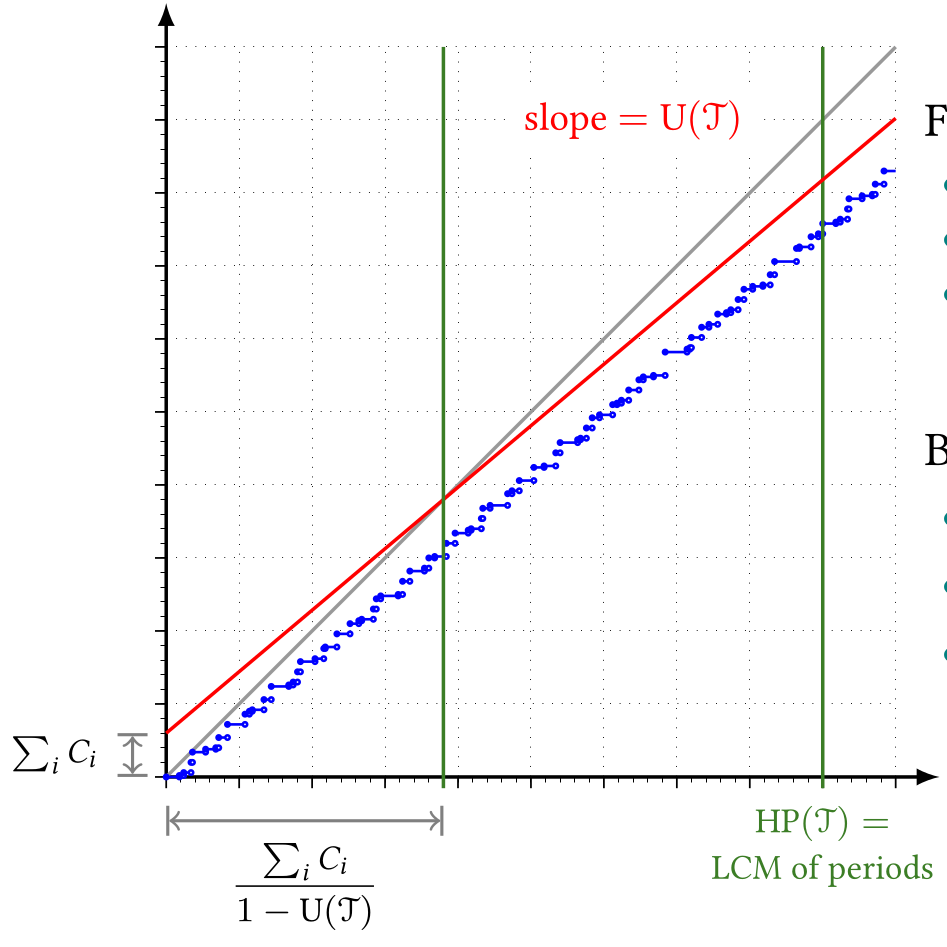
\includegraphics[width=10cm]{\imagesPath/dbf.png}
    \caption{DBF graph}
    \label{fig:dbf}
\end{figure}

The hyper period is calculated by finding the least common multiple. 
This only work for a shedable processor.
\begin{exampleblock}{Hyper period}
  Let task set $\mathcal{J}= \{(2,7,8),(4,8,9),(3,10,10)\}$
  \begin{align*}
    8 &= 2\cdot2\cdot2 \\
    9 &= 3\cdot3 \\ 
    10 &= 5\cdot2 \\
  \end{align*}
  Then the hyper period is:
  \begin{equation*}
    2\cdot2\cdot2\cdot3\cdot3\cdot5 = 4\cdot9\cdot10 = 36\cdot10 = 360  
  \end{equation*}
\end{exampleblock}

\begin{exampleblock}{dbf}
%  $T_i=(2,3,5)$
%  \begin{align*}
%    dbf(1) &= L \frac{1-3}{5} + 1)2 = 0  \\ %start with 1 then 2 and so on for all $t_i$
%    dbf(2) &= ([\frac{-1}{5}+1])2=0 \\
%    dbf(3) &= (0+1)2=2 \\
%    dbf(7) &= ([\frac{4}{5}]+1)2=2 \\
%    dbf(8) &= ([\frac{5}{5}]+1)2=4 \\
%  \end{align*}
  Then draw it out with will be stepwise function with define length of each lines. each step is one unit in between (the y-axis)

  Don't need to test all, there is a bound only up to the Hyper period plus max relative deadline
\end{exampleblock}

If all deadlines are implicit it is a lot easier whe need just to check that the total utilization is less then 1 see the formula above for utilization.



\subsection{Jitter}

Jitter can be due to Tick-driven scheduler, since the timing-interupps accures every 10th ms 
so we could be unlocky and have 10ms jitter.

varying execution time that start another task is another source of jitter

Jitter, not exact or other tasks
\begin{align*}
  R_i &= \mathpzc{w}_i + \mathpzc{J}_i \\
  \mathpzc{w}_i &= C_i + \sum_{j \in hp(\tau_i)} \left\lceil\frac{\mathpzc{w}_i + \mathpzc{J}_j}{T_j}\right\rceil C_j \\
\end{align*}
an optimistic view, so we can see the maximum allowed jitter

%finding the executing time, we need since deadline and priotiry we have. We cant define it but we can have a estimate.


\section{Workload Models}
Several real-time systems contain functionality of different 
\textit{importance}, or \textit{criticality}. 
Such systems are sometimes called mixed-criticality systems.

In such system let every task $\tau_i$ have two WCET estimates
$C_i^{HI}$, pesimistic estimation, and $C_i^{LO}$, not pesimistic estimation. 
\begin{equation}
  C_i^{LO} \leq C_i^{HI} 
\end{equation}
Were the criticality level $\chi_i\in\{LO, HI\}$, i.e \{ Low citicality, High criticality\}.


\begin{exampleblock}{Criticality}
  Let,
  \begin{align*}
    \mathcal{J} &= \{\tau_1, \tau_2, \tau_3\} \\
    &= \{ (1,1,HI,4,4), (1,2,HI,3,4), (3,3,LO,9,10) \}
  \end{align*}

  Then the critical instance schedule will use only the HI value 
  when locking at WCET for a task and only on the LO for task with 
  low criticality. See Figure \ref{fig:mixed-criticality_HI} and Figure 
  \ref{fig:mixed-criticality_LO}.
\end{exampleblock}

\begin{figure}[H]
    \centering
    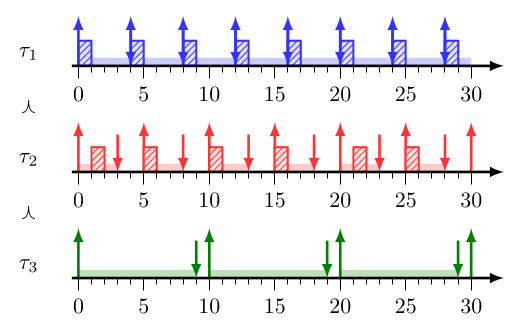
\includegraphics[width=10cm]{\imagesPath/mixed-criticality_HI.png}
    \caption{Timing Constraints, \cite{08A-advanced-workload-model, p.11}}
    \label{fig:mixed-criticality_HI}
\end{figure}

\begin{figure}[H]
    \centering
    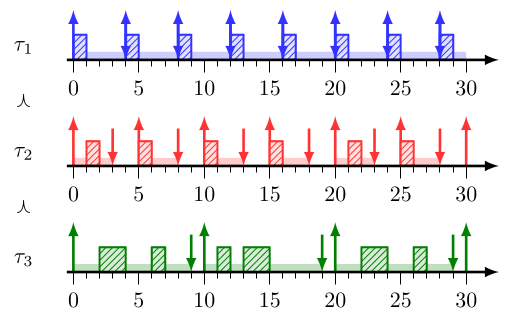
\includegraphics[width=10cm]{\imagesPath/mixed-criticality_LO.png}
    \caption{Timing Constraints, \cite{08A-advanced-workload-model, p.11}}
    \label{fig:mixed-criticality_LO}
\end{figure}

\textbf{Correctness criteria for mix-criticality}. We say that scheduling is correct iff
\begin{enumerate}
  \item All jobs meet their deadlines when all actual
        execution times stay below the $C_i^{LO}$'s in the current
        run of the system.
  \item Jobs from high-criticality tasks meet their deadlines
        when all actual execution times stay below the $C_i^{HI}$'s
        in the current run of the system.
\end{enumerate}

Schedulable test
\begin{equation}
  R_i = C_i^{\chi_i} + \sum_{\tau\in hp(\tau_i)} \left\lceil \frac{R_i}{T_j} \right\rceil C_j^{\chi_i}
\end{equation}


%Have complexity graph here
Not all sets of tasks are sporadic.
\begin{itemize}
  \item The general multiframe (GMF) Task Model: cyrclic
  \item The Recurring Branching (RB) Task model: diffrent branches
  \item The Digraph real-time model (DRT): diffrent branches and circles
\end{itemize}

\begin{figure}[H]
    \centering
    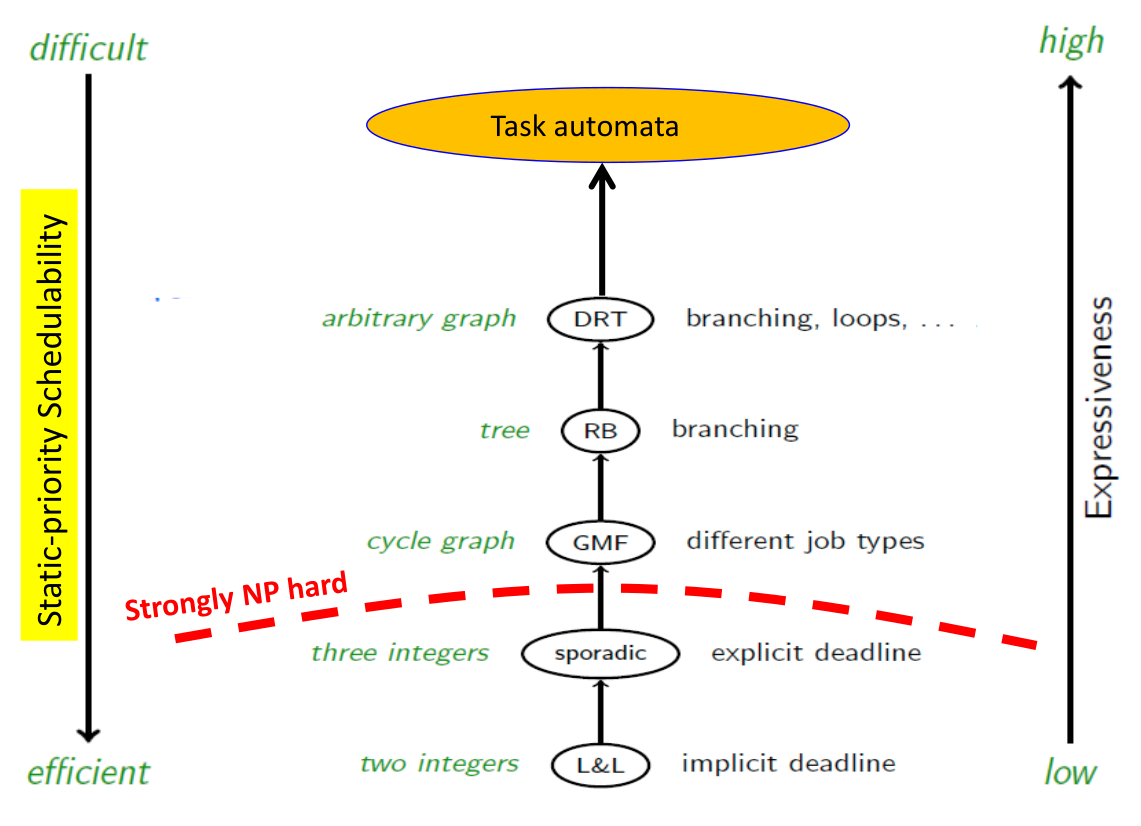
\includegraphics[width=10cm]{\imagesPath/hierarchy_of_models.png}
    \caption{Hierarchy of Models}
\end{figure}


Demand Bound Function (DBF). 
$C_{max}$ add up every execution demand, i.e. the first ellement of the demand pair for all elements in the task model.



\section{Synchronization}

\subsection{Blocking}
Blocking occurs when one or more lower priority task uses a semaphore that a higher priority task wants,
thus worsen the WCRT. 

If we allow blocking, then the worst case execution time is:
\begin{equation}
  R_i = C_i + B_i + \sum_{j \in hp(i)} \left\lceil \frac{R_i}{T_j} \right\rceil C_j
\end{equation}

Un-bounded priority inversion occurs when a lower priority task has taken
the semaphore and it is not allowed to run since a higher priority task
is running, which is lower priority task then the task who wants the semaphore.

To solve priority inversion there are a few resource access protocols.
\begin{itemize}
  \item Highest Priority Inheritance
  \begin{itemize}
    \item Non preemption protocol (NPP)
  \end{itemize}
  \item Basic Priority Inheritance Protocol (BIP)
  \begin{itemize}
    \item POSIX (RT OS standard) mutexes
  \end{itemize}
  \item Immedate Priority Inheritance
  \begin{itemize}
    \item Highest Locker's priority Protocol (HLP)
    \begin{itemize}
      \item Ada95 (protected object) and POSIX mutexes
    \end{itemize}
  \end{itemize}
  \item Priority Ceiling Protocols (PCP)
  \begin{itemize}
    \item The general one
  \end{itemize}
\end{itemize}


\subsection{Non preemption protocol (NPP)}
%Assigns the higher priority of the caller using the semaphore to 
%the user of the semaphore.
The one who successfully grabs the semaphore will get the highest priority.
Meaning that it will not be preempted as no other task has higher priority.
However, lower priority task will then block higher priority tasks.

%\textbf{image}
%\textbf{code}


\subsection{Basic Priority Inheritance Protocol (BIP)}
The one who tries to get a semaphore that another already have taken will swhich priorites.

\begin{itemize}
  \item A gets semaphore S
  \item B with higher priority tries to lock S, but cant since A has it
  \item B transfers its priority to A, so that A runs with B's priority.
\end{itemize}

\textbf{image}
\textbf{code}
\begin{verbatim}
P(scb):
  Disable-interrupt;
  If scb.counter>0 then {scb.counter - -1;
                         scb.holder:= current-task
                         add(current-task.sem-list,scb)}
  else
    {save-context( );
    current-task.state := blocked;
    insert(current-task, scb.queue);
    save(scb.holder.priotiry);
    scb.holder.priority := current-task.priority;
    schedule();
    load-context() }
  Enable-interrupt
\end{verbatim}

\begin{verbatim}
V(scb):
  Disable-interrupt;
    Restore current-task.priority (with ”its original priority”)
    If not-empty(scb.queue) then
      { next-to-run := get-first(scb.queue);
        scb.holder := next-to-run;
      next-to-run.state := ready;
      insert(next-to-run, ready-queue);
      save-context();
      schedule();
      load-context() }
    else scb.counter ++1;
  Enable-interrupt
\end{verbatim}

\begin{figure}[H]
    \centering
    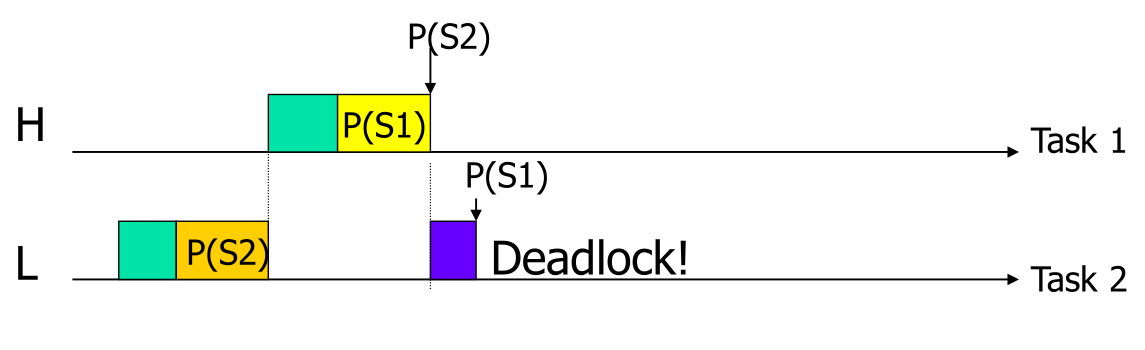
\includegraphics[width=10cm]{\imagesPath/bip_deadlock.png}
    \caption{Potential deadlock with BIP scheduling}
\end{figure}


\subsection{Immedate Priority Inheritance and HLP}
The task that grabs the semaphore will directly get the priority which is assigned 
to that semaphore.

\begin{figure}[H]
    \centering
    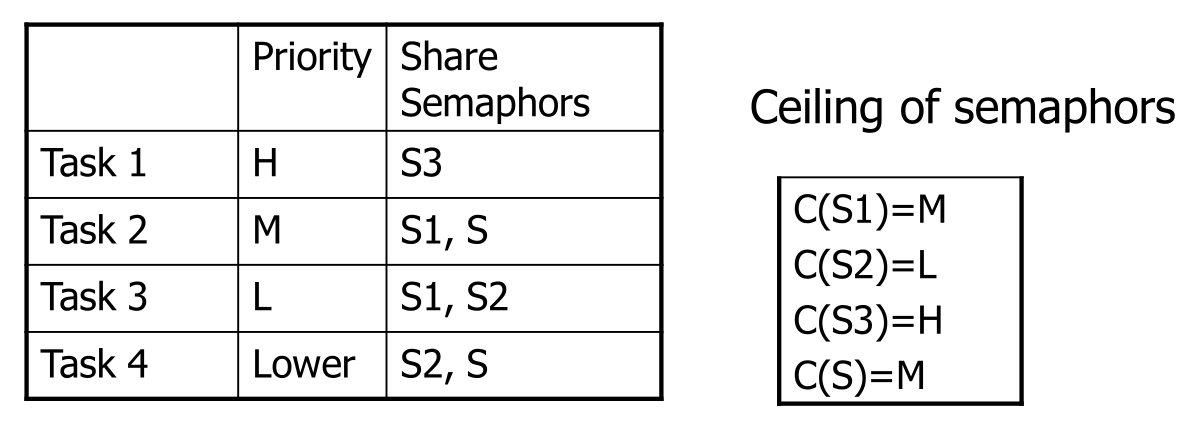
\includegraphics[width=10cm]{\imagesPath/hlp_example.png}
    \caption{HLP example of ceiling table}
\end{figure}

%If we use the priority inharitance protocal, where a task will inherit the priority of the task that the lock which the task is waiting for
%$B_i$ is calculated by extreacting the maximum time of any lower priority task that is accessing the semaphore.
%We dont need to calculate for those with higher priority since they already are counted in the sum

\begin{verbatim}
P(scb):
  Disable-interrupt;
    If scb.counter>0 then
      { scb.counter - -1;
        current-task.priority := Ceiling(scb) }
    else
      { save-context();
        current-task.state := blocked
        insert(current-task, scb.queue);
        schedule();
        load-context() }
  Enable-interrupt
\end{verbatim}

\begin{verbatim}
V(scb):
  Disable-interrupt;
  Restore current-task.priority
  If not-empty(scb.queue) then
    next-to-run := get-first(scb.queue);
    next-to-run.state := ready
    insert(next-to-run, ready-queue);
    save-context();
    schedule(); /* dispatch invoked*/
    load-context();
  end then
  else scb.counter ++1;
  end else
  Enable-interrupt
\end{verbatim}


\subsection{Priority Ceiling Protocols (PCP)}
PCP is an extension of PIP and HLP.



\begin{table}[H]
  \centering
\begin{tabular}{ |c|c|c|c|c| } 
  \hline
                             & NPP  & BIP  & HLP    & PCP \\
  \hline
  Bounded Priority Inversion & yes  & yes  & yes    & yes \\
  \hline
  Deadlock free              & yes  & no   & yes    & yes \\
  \hline
  Un-necessary blocking      & yes  & no   & yes/no & no \\
  \hline
  Blocking time calculation  & easy & hard & easy   & easy \\
  \hline
  Number of blocking         & $1$  & $>1$ & $1$    & $1$ \\
  \hline
  Implementation             & easy & easy & easy   & hard \\
  \hline
\end{tabular}
\end{table}


\section{Multiprocessor scheduling}

\subsection{Multiprocessor Scheduling of Task Graphs}
The response time will is bounded with graham' bound
\begin{align*}
  R \leq len(G) + \frac{vol(G) - len(G)}{m}
\end{align*}
Where $len(G)$ is the lenght of the longest path, $vol(G)$ is the 
total workload, and $m$ is the number of processors. This is somewhat 
logical bound since we know that $R \geq len(G)$ and to get the work case 
we need to add the workload that could theorieiclay be scheduled before 
the jobs in the longest path.

Utilization bound
\begin{itemize}
  \item Global Scheduling: formula? 
  \item Partitioned Scheduling: 50\% for each queue?
  \begin{itemize}
    \item First Fit manner: highest priority first.
  \end{itemize}
  \item Partitioned Scheduling with Task Splitting: 
  \begin{itemize}
    \item Lakshmanan' algorithm: 65\% for each queue
    \item breadth-first partitioning algorithm: 69\% for each queue (same as RM)
    \item preasigning heavy task: $\frac{C_i/T_i}{M} \leq N(2^{1/N}-1)$
  \end{itemize}
\end{itemize}

Heavy task is tasks with utilization higher than 0.41.

Advantages and disadvantages for scheduling algorithms
\begin{itemize}
  \item Global Scheduling:
  \begin{itemize}
    \item (+) Supported by most multiprocessor os. 
    \item (-) No optimal algorithm  
    \item (-) Poor resource utilization for hard RT.
    \item (-) Experiances sheduling anomalis
  \end{itemize}
  \item Partitioned scheduling:
  \begin{itemize}
    \item 
  \end{itemize}
  \item Partitioned scheduling with task splitting:
  \begin{itemize}
    \item (+) Better resource utilization.
    \item (-) Task splitting requires more preemption and migration.
  \end{itemize}
\end{itemize}


\subsection{Multiprocessor Scheduling of Task Graphs}
\begin{figure}[H]
    \centering
    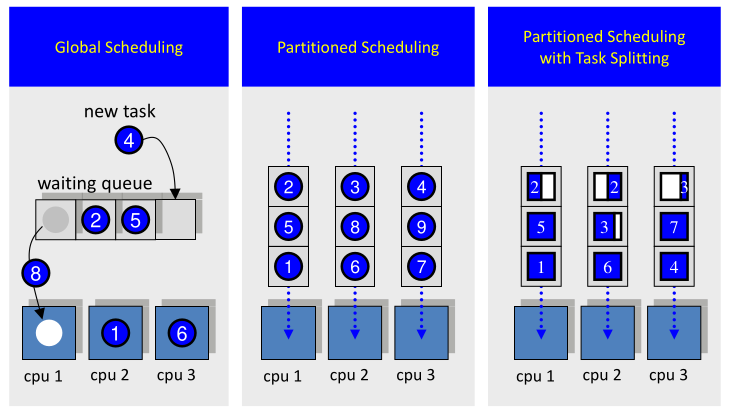
\includegraphics[width=10cm]{\imagesPath/multiprocessor_scheduling_of_sequantial_tasks.png}
    \caption{Multiprocessor Scheduling of sequential tasks, \cite{11-multiprocessor-2, p.6}}
    \label{multiprocessor_scheduling_of_sequantial_tasks}
\end{figure}

EDF is not optimal, Fixed priority suffers from Dhall's anomali. 
Dhall's anomali happens for instance when there is 3 tasks that are
scheduled on 2 cpu's and the shortest jobs will be scheduled first thus
the longer job will be scheduled after a shorther job thus worsening the 
WCET.

There is also Richard's anomali, increasing the number of processors 
might make the schedule wors.

\begin{figure}[H]
    \centering
    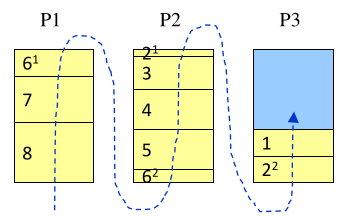
\includegraphics[width=10cm]{\imagesPath/lakshmanan's_algorithm.png}
    \caption{Lakshmanan's Algorithm, \cite{11-multiprocessor-2, p.6}}
    \label{lakshmanan's_algorithm}
\end{figure}

\begin{figure}[H]
    \centering
    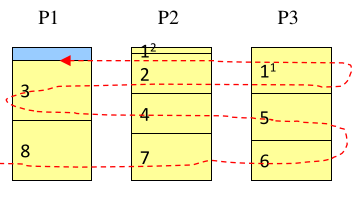
\includegraphics[width=10cm]{\imagesPath/breadth-first_partiononing_algorithms.png}
    \caption{breadth-first partiononing algorithms, \cite{11-multiprocessor-2, p.6}}
    \label{breadth-first_partiononing_algorithms}
\end{figure}

There is also a solution to assigning tasks to queses with the heavy tasks first.
Meaning that if the task is significantly larger then the others it will be 
assign to a queue first. It is called pre-assigning the heavy tasks.


\section{UPPAAL}
\begin{itemize}
  \item ! (shoting I want to do somthing)
  \item ? (does somwan want to do somthign) If we shout somone needs to answer.
  \item E (some exectuion of our system)
  \item A (one posible exectution)
  \item <> (some point in the execution)
  \item [] (all parts of the exectuion)
\end{itemize}

There will alwaes be a deadlock if all tasks can reach a done state there fore to check if no deadlock occurs
we need to check that there is no state where there is a deadlock and all tasks has not reached there done state.
\begin{center}
  \texttt{A[] not (deadlock and prod\_done==false and cons\_done==false and buff\_done==false)}
\end{center}

\section{Real time communication (RTC)}
Can bus is one of the most common forms of real time communication, since of the low cost and dependability.
It is chared broadcast meaing that you dont send a message to a spesific node but broadcasts it and those who are intreased will listen.
The arbitration mechanism shown in Figure \ref{can_arbitration_mechanism}, allowes the node with the highest priority send first.
The priority is dependent on the identifier. It is there fore important not to have the same identifier or the behaviur will be unexpected.
\begin{figure}[H]
    \centering
    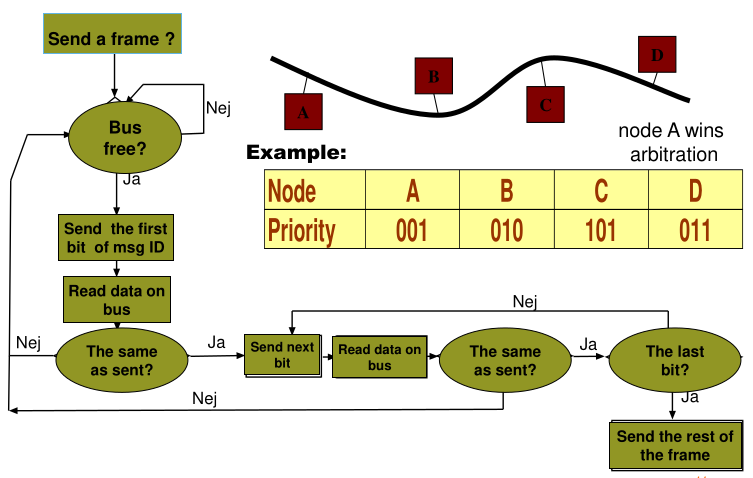
\includegraphics[width=10cm]{\imagesPath/can_arbitration_mechanism.png}
    \caption{CAN Arbitration Mechanism, \cite{14-rtc, p.11}}
    \label{can_arbitration_mechanism}
\end{figure}


\begin{table}[H]
  \centering
\begin{tabular}{ |p{1cm}|p{1.4cm}|p{1cm}|p{1.1cm}|p{1cm}|p{1cm}|p{1cm}|p{1cm}|p{1cm}|p{1cm}|p{1cm}| } 
  \hline
  SOF, Start Of Frame & 
  Identifier &
  RTR, Remote Transition Request &
  Control &
  Data &
  CRC, Cyclic Redundancy Check &
  CRC DEL, CRC Delimiter &
  ACK, Acknowledge &
  ACK DEL, Acknowledge Delimiter &
  EOF, End of Frame &
  IFS, Inter Frame Space \\
  \hline
  1 bit & 
  11 bits &
  1 bit &
  6 bits &
  0-8 bytes &
  15 bits &
  1 bit &
  1 bit &
  1 bit &
  7 bits &
  3$-$, min 3 bits \\
  \hline
\end{tabular}
  \caption{Note that the field priority/idenfitier}
\end{table}

The maximum size is:
\begin{equation*}
  64 \text{bits} + 47 \text{bits} + 24 \text{bits} = 135 \text{bits}
\end{equation*}
if the message is sent 1Mbit/sec then the max transmition time for one message is $135$ microseconds.

Task "comp" to produce a message at A:
\begin{align*}
  X_{comp} &= C_{comp} + \sum_{j\in hp(comp)} \left\lceil \frac{(X_{comp} + J_j)}{T_j} \right\rceil C_j \\ 
  R_{comp} &= X_{comp}^* + J_{comp}
\end{align*}

Task "send" to transmit the message at A:
\begin{align*}
  J_{send} &= R_{comp} - C_{comp} \\
  Y_{send} &= C_{send} + B_{send} + \sum_{j\in hp(send)} \left\lceil \frac{(Y_{send} + J_j)}{T_j} \right\rceil C_j \\
  R_{send} &= Y_{send}^* + J_{send} = Y_{send}^* + R_{comp}
\end{align*}

Task "dest" to consume the message at B:
\begin{align*}
  J_{dest} &= R_{send} - C{send} \\
  Z_{dest} &= C_{dest} + \sum_{j\in hp(dest)} \left\lceil \frac{(Z_{dest} + J_j)}{T_j} \right\rceil C_j \\
  R_{dest} &= Z_{dest}^* + J_{dest} = Z_{dest}^* + R_{send}
\end{align*}

$C_{send}=B_{send}=$ 135 mico sec if message size is 135 bits